\documentclass{article}

\usepackage[margin=0.5in]{geometry}
\usepackage{tikz}
\usepackage{amsmath}
\usepackage{pgfplots}
\usepackage{gensymb}

\pgfplotsset{compat=1.17}

\title{Year 5 Mathematics Mock Exam}
\author{Aldrine Einsteen}
\date{}

\begin{document}

\maketitle

\section*{Instructions}
This exam consists of seven sections. You have 60 minutes to complete the exam. Do not use a calculator.

\section{Arithmetic}
1. If $a=2$, $b=3$, and $c=4$, evaluate: $2a + 3b - 4c$. \\
2. Simplify: $7(3x+4)-2(5x-3)$. \\
3. What is the product of $7$ and $9$? \\

\section{Number and Place Value}
1. Write the number $5,678$ in words. \\
2. What is the value of the '5' in $125,463$? \\
3. Write 'four hundred and twenty three thousand and thirty two' in figures. \\

\section{Fractions}
1. Simplify $\frac{14}{28}$. \\
2. What is $\frac{1}{2}$ of $\frac{2}{3}$? \\
3. Subtract $\frac{2}{5}$ from $\frac{3}{4}$. \\

\section{Decimals}
1. Write the decimal $0.625$ as a fraction. \\
2. Round $7.86$ to the nearest whole number. \\
3. Add $1.2$ and $3.56$. \\

\section{Percentages}
1. What is $20\%$ of $50$? \\
2. Convert $45\%$ to a decimal. \\
3. Express $\frac{1}{5}$ as a percentage. \\

\section{Measurement and Geometry}
1. If the radius of a circle is $5$ cm, calculate the area. (Use $\pi = 3.14159$) \\
2. Find the perimeter of a rectangle with length $6$ cm and width $4$ cm. \\
3. A triangle has a base of $8$ cm and a height of $5$ cm. What is its area? \\

\section{Graphs and Bar Charts}
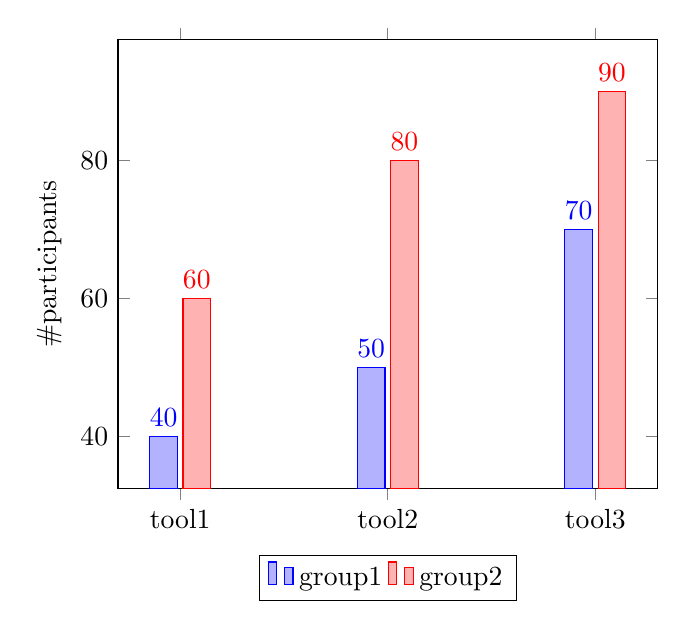
\begin{tikzpicture}
\begin{axis}[
    ybar,
    enlargelimits=0.15,
    legend style={at={(0.5,-0.15)},
      anchor=north,legend columns=-1},
    ylabel={\#participants},
    symbolic x coords={tool1,tool2,tool3},
    xtick=data,
    nodes near coords,
    nodes near coords align={vertical},
    ]
\addplot coordinates {(tool1,40) (tool2,50) (tool3,70)};
\addplot coordinates {(tool1,60) (tool2,80) (tool3,90)};
\legend{group1,group2}
\end{axis}
\end{tikzpicture}

1. How many participants used tool1 in group1? \\
2. Which tool was used by the most participants in group2? \\
3. How many more participants used tool3 than tool2 in group1? \\

\end{document}
